
% Copyright 2004 by Till Tantau <tantau@users.sourceforge.net>.
%
% In principle, this file can be redistributed and/or modified under
% the terms of the GNU Public License, version 2.
%
% However, this file is supposed to be a template to be modified
% for your own needs. For this reason, if you use this file as a
% template and not specifically distribute it as part of a another
% package/program, I grant the extra permission to freely copy and
% modify this file as you see fit and even to delete this copyright
% notice. 

\documentclass{beamer}

% There are many different themes available for Beamer. A comprehensive
% list with examples is given here:
% http://deic.uab.es/~iblanes/beamer_gallery/index_by_theme.html
% You can uncomment the themes below if you would like to use a different
% one:
%\usetheme{AnnArbor}
%\usetheme{Antibes}
%\usetheme{Bergen}
%\usetheme{Berkeley}
%\usetheme{Berlin}
%\usetheme{Boadilla}
%\usetheme{boxes}
%\usetheme{CambridgeUS}
%\usetheme{Copenhagen}
%\usetheme{Darmstadt}
%\usetheme{default}
%\usetheme{Frankfurt}
%\usetheme{Goettingen}
%\usetheme{Hannover}
%\usetheme{Ilmenau}
%\usetheme{JuanLesPins}
%\usetheme{Luebeck}
\usetheme{Madrid}
%\usetheme{Malmoe}
%\usetheme{Marburg}
%\usetheme{Montpellier}
%\usetheme{PaloAlto}
%\usetheme{Pittsburgh}
%\usetheme{Rochester}
%\usetheme{Singapore}
%\usetheme{Szeged}
%\usetheme{Warsaw}

\title{Session 2}

% A subtitle is optional and this may be deleted
\subtitle{Recognizing Handwritten Digits}

%\author{F.~Author\inst{1} \and S.~Another\inst{2}}
% - Give the names in the same order as the appear in the paper.
% - Use the \inst{?} command only if the authors have different
%   affiliation.

\institute[Computer Vision Group]
{
  Computer Vision Group\\
  IIT Madras
}  
\date{December 2, 2014}
% - Either use conference name or its abbreviation.
% - Not really informative to the audience, more for people (including
%   yourself) who are reading the slides online

\subject{Theoretical Computer Science}
% This is only inserted into the PDF information catalog. Can be left
% out. 

% If you have a file called "university-logo-filename.xxx", where xxx
% is a graphic format that can be processed by latex or pdflatex,
% resp., then you can add a logo as follows:

% \pgfdeclareimage[height=0.5cm]{university-logo}{university-logo-filename}
% \logo{\pgfuseimage{university-logo}}

% Delete this, if you do not want the table of contents to pop up at
% the beginning of each subsection:
%\AtBeginSubsection[]
%{
%  \begin{frame}<beamer>{Outline}
%    \tableofcontents[currentsection,currentsubsection]
%  \end{frame}
%}

% Let's get started
\begin{document}

\begin{frame}
  \titlepage
\end{frame}

\begin{frame}{Outline}
  \tableofcontents
  % You might wish to add the option [pausesections]
\end{frame}

% Section and subsections will appear in the presentation overview
% and table of contents.
\section{Feature Extraction}

\subsection{Observing MNIST dataset}
\begin{frame}{Observing MNIST dataset}{Feature Extraction}
    \begin{block}{Training set}
        Unzip the file training.zip. We'll use contents of the extracted folder to train
        our classifier.
    \end{block}
    \begin{block}{Test set}
        Unzip the file test.zip. We'll use the contents of the extracted folder to test
        the performance of our classifier.
    \end{block}

    \begin{block}{Observe the 10 folders}
        Each folder has images of a particular handwritten digit. 
    \end{block}
\end{frame}

\subsection{Saving features to a file}

% You can reveal the parts of a slide one at a time
% with the \pause command:
\begin{frame}{Saving features to a file}{Feature Extraction}
  \begin{itemize}
  \item{
    Each image is of dimension 28 x 28. (Thats 28 x 28 = 784 pixel values)
  }
  \pause
  \item{   
    Use pixel access to save each pixel intensity to a file in the csv format.
  }
  \pause
  \begin{block}{CSV format}
      Traverse through each image in the row-major form and store the values seperated by
      a comma. Each line in the file will correspond to features from a single image.
      \begin{example}
        A CSV form of five 28 x 28 images will have 5 lines, with each line containing
        (28 x 28 - 1) commas.
      \end{example}
  \end{block}
  \pause
  \item You should now have two files, namely train.csv and test.csv which contain data 
  corresponding to the training and test datasets.
  \end{itemize}
\end{frame}

\section{Training a classifier}

\subsection{Support Vector Machines}
\begin{frame}{Support Vector Machines}{Training a Classifier}
    \centering
        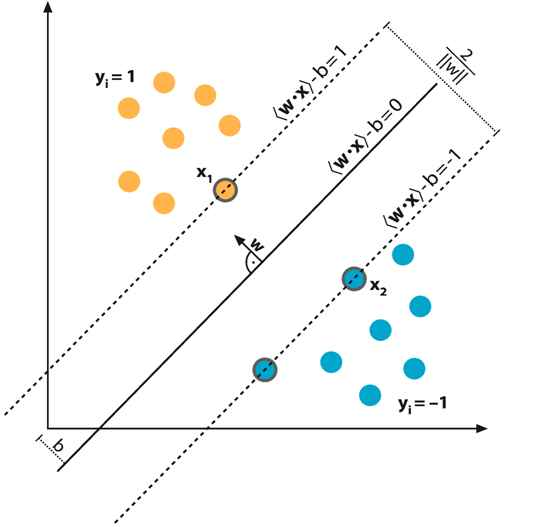
\includegraphics[width=50mm]{./images/svm.jpg}

\begin{itemize}
    \item They find an optimal seperation between classes.
    \item OpenCV has inbuilt functions to implement this classfier.
\end{itemize}
\end{frame}

\subsection{Implementing an SVM}
\begin{frame}{Implementing an SVM}{Training a classifier}
    \centering
       \textbf{Hands on}\\
\end{frame}

\section{Testing the classifier}
\subsection{Using the classifier on new images}
\begin{frame}{Using the classifier on new images}{Testing the classifier}
    \centering
        \textbf{Hands on}\\
\end{frame}

\subsection{Evaluation Measure}
\begin{frame}{Evaluation Measure - Misclassification rate}{Testing the classifier}
    Since its a classification task (image is being classified as one of 10 digits), 
    misclassification rate could be used as a criterion for evaluating the performance of
    the classifier.
   
    \begin{block}{Other performance measures}
    \begin{itemize}
    \item Precision
    \item Recall
    
    \end{itemize}
    \end{block}

\end{frame}
% Placing a * after \section means it will not show in the
% outline or table of contents.

\section{Scope for improvement}
\begin{frame}{Scope for improvement}
\begin{itemize}
\item Feature Extraction?
\pause
\item Reducing the number of features?
\pause
\item Better classifier?
\end{itemize}

\end{frame}
\section*{Summary}
\begin{frame}{Summary}
    \begin{block}{Today's session}
        We successfully built a handwritten gesture recongition. We also learnt
        about support vector machines.
    \end{block}
    \begin{block}{Tomorrow's session}
        \begin{itemize}
        \item \textbf{Segmenting out digits} using the classfier we built today. 
        \item We used cropped images to train our classifier today. What if there are 
        many digits in the image? How do we automatically find out the parts of the 
        image which contain digits?
        \end{itemize}
    \end{block}
\end{frame}

\end{document}


